\documentclass[a4paper,12pt]{article}

% Paquetes básicos
\usepackage[utf8]{inputenc}
\usepackage[T1]{fontenc}
\usepackage[spanish]{babel}
\usepackage{graphicx}
\usepackage{xcolor}
\usepackage{lipsum}
\usepackage{geometry}
\geometry{top=3cm, bottom=3cm, left=2.5cm, right=2.5cm}

% Paquetes para diseño
\usepackage{titlesec}
\usepackage{fancyhdr}
\usepackage{amsmath}
\usepackage{amssymb}
\usepackage{hyperref}
\usepackage{enumitem}
\usepackage{float}
\usepackage{multicol}
\usepackage{listings}
\usepackage{color}
\usepackage{tcolorbox}

% Paquetes para el entorno lstlisting
\usepackage{listings}
\usepackage{inconsolata}

%encabezado y pie de página nivel profesional
\usepackage{fancyhdr}
\pagestyle{fancy}
\fancyhf{}
\fancyhead[L]{\leftmark}
\fancyhead[R]{\rightmark}
\fancyfoot[L]{\textit{Ismael Sallami Moreno - GIIADE}}
\fancyfoot[C]{\thepage}
\fancyfoot[R]{\textbf{(UGR)} \today}
\renewcommand{\headrulewidth}{0.4pt}
\renewcommand{\footrulewidth}{0.4pt}
\setlength{\headheight}{15pt}
\setlength{\headsep}{10pt}
\setlength{\footskip}{20pt}
\usepackage{truncate}
\fancyhead[L]{\truncate{0.5\headwidth}{\leftmark}}
\fancyhead[R]{\truncate{0.5\headwidth}{\rightmark}}
\usepackage{mathpazo}
% Paquete para fondo
\usepackage{background}

% Configuración de lstlisting
\lstset{
    inputencoding=utf8,          % Permite UTF-8
    extendedchars=true,          % Reconoce caracteres extendidos
    literate=                    % Configuración manual para tildes y símbolos
        {á}{{\'a}}1
        {é}{{\'e}}1
        {í}{{\'i}}1
        {ó}{{\'o}}1
        {ú}{{\'u}}1
        {ñ}{{\~n}}1
        {Á}{{\'A}}1
        {É}{{\'E}}1
        {Í}{{\'I}}1
        {Ó}{{\'O}}1
        {Ú}{{\'U}}1
        {Ñ}{{\~N}}1
        {¿}{{\textquestiondown}}1
        {¡}{{\textexclamdown}}1,
    basicstyle=\ttfamily,        % Fuente monoespaciada
    breaklines=true,             % Habilita salto de línea automático
    frame=single,                % Marco alrededor del código
    backgroundcolor=\color{gray!10}, % Fondo gris claro
    keywordstyle=\color{blue},   % Color para palabras clave
    commentstyle=\color{green},  % Color para comentarios
    stringstyle=\color{red}      % Color para strings
}
\lstdefinestyle{customcpp}{
    language=C++,                % Lenguaje de programación
    showspaces=false,            % No mostrar espacios
    showtabs=false,              % No mostrar tabulaciones
    tabsize=4,                   % Tamaño de tabulación
    showstringspaces=false,      % No mostrar espacios en strings
    numbers=left,                % Números de línea a la izquierda
    numberstyle=\tiny\color{gray}, % Estilo de los números de línea
    numbersep=5pt,               % Separación de los números de línea
    stepnumber=1,                % Mostrar número en cada línea
    basicstyle=\ttfamily\footnotesize, % Estilo básico del código
    keywordstyle=\bfseries\color{blue}, % Estilo de las palabras clave
    commentstyle=\itshape\color{green!50!black}, % Estilo de los comentarios
    stringstyle=\color{red},     % Estilo de los strings
    identifierstyle=\color{black}, % Estilo de los identificadores
    % procnamekeys={def,class},    % Palabras clave para nombres de funciones
    morekeywords={constexpr,nullptr,size_t}, % Más palabras clave
    emph={int,char,double,float,unsigned}, % Palabras a enfatizar
    emphstyle=\color{magenta},   % Estilo de las palabras enfatizadas
    backgroundcolor=\color{gray!10}, % Color de fondo
    frame=shadowbox,             % Marco con sombra
    rulesepcolor=\color{gray},   % Color de la línea de separación
    breakatwhitespace=false,     % No cortar en espacios en blanco
    breaklines=true,             % Cortar líneas largas
    captionpos=b,                % Posición del título (abajo)
    escapeinside={(*@}{@*)},     % Delimitadores para escapar a LaTeX
    morecomment=[l][\color{magenta}]{\#}, % Comentarios de una línea
    morecomment=[s][\color{orange}]{/*}{*/}, % Comentarios multilínea
    morestring=[b]",             % Strings entre comillas dobles
    morestring=[b]'              % Strings entre comillas simples
}

% Configuración de título
\titleformat{\section}{\normalfont\Large\bfseries}{\thesection}{1em}{}

% Información del documento
\title{
    \vspace{-2cm}
    
\includegraphics[width=0.3\textwidth]{images/etsiit.png} \\ % Cambia el logo si es necesario
    \LARGE Ingeniería Informática + ADE\\
    \large Universidad de Granada (UGR)\\[1cm]
}
\author{\textbf{Autor:} Ismael Sallami Moreno}
\date{\textbf{Asignatura:} Ejercicios Tema 3 SCD: Paso de mensajes}

% Configuración del fondo
\backgroundsetup{
    scale=1,
    color=black,
    opacity=0.2,
    angle=0,
    position=current page.south,
    vshift=0pt,
    hshift=0pt,
    contents={
\includegraphics[width=\paperwidth,height=\paperheight,keepaspectratio]{images/granada.jpg}}
}

% Inicio del documento
\begin{document}

% Portada
\maketitle
\thispagestyle{empty}

\begin{center}
    
\includegraphics[width=\textwidth,height=0.4\textheight,keepaspectratio]{images/granada.jpg} \\ % Añade tu imagen de fondo
    \vfill
\end{center}

\newpage

% Índice (opcional)
\tableofcontents
\newpage
\section{Ejercicio 77}

\subsection{Enunciado}
En un sistema distribuido, 6 procesos clientes necesitan sincronizarse de forma específica para
realizar cierta tarea, de forma que dicha tarea sólo podrá ser realizada cuando tres procesos estén
preparados para realizarla. Para ello, envían peticiones a un proceso controlador del recurso y
esperan respuesta para poder realizar la tarea específica. El proceso controlador se encarga
de asegurar la sincronización adecuada. Para ello, recibe y cuenta las peticiones que le llegan
de los procesos, las dos primeras no son respondidas y producen la suspensión del proceso
que envía la petición (debido a que se bloquea esperando respuesta) pero la tercera petición
produce el desbloqueo de los tres procesos pendientes de respuesta. A continuación, una vez
desbloqueados los tres procesos que han pedido (al recibir respuesta), inicializa la cuenta y
procede cíclicamente de la misma forma sobre otras peticiones. El código de los procesos
clientes aparece aquí abajo. Los clientes usan envío asíncrono seguro para realizar su petición,
y esperan con una recepción síncrona antes de realizar la tarea:

\begin{lstlisting}[style=customcpp]
process Cliente[ i : 0..5 ] ;
begin
  while true do begin
    send( peticion, Controlador );
    receive( permiso, Controlador );
    Realiza_tarea_grupal();
  end
end

process Controlador ;
begin
  while true do begin
    ...
  end
end
\end{lstlisting}

Describir en pseudocódigo el comportamiento del proceso controlador, utilizando una orden de
espera selectiva que permita implementar la sincronización requerida entre los procesos. Es
posible utilizar una sentencia del tipo select for i=... to ... para especificar diferentes ramas de una sentencia selectiva que comparten el mismo código dependiente del valor
de un índice i.

\subsection{Solucion}

En un sistema distribuido, 6 procesos clientes necesitan sincronizarse de forma específica para realizar cierta tarea, de forma que dicha tarea sólo podrá ser realizada cuando tres procesos estén preparados para realizarla. Para ello, envían peticiones a un proceso controlador del recurso y esperan respuesta para poder realizar la tarea específica. El proceso controlador se encarga de asegurar la sincronización adecuada. 

El controlador cuenta las peticiones que le llegan de los procesos:
\begin{itemize}
    \item Las dos primeras peticiones no son respondidas, lo que provoca que los procesos que las envían queden bloqueados esperando una respuesta.
    \item La tercera petición produce el desbloqueo de los tres procesos pendientes, enviándoles una respuesta.
\end{itemize}

Una vez desbloqueados los tres procesos, el controlador inicializa la cuenta y procede cíclicamente de la misma forma para nuevas peticiones. Los clientes usan envío asíncrono seguro para realizar su petición y esperan con una recepción síncrona antes de realizar la tarea.

El código de los procesos clientes es el siguiente:

\begin{lstlisting}[style=customcpp, caption={Código de los procesos clientes}]
process Cliente[ i : 0..5 ] ;
begin
  while true do begin
    send( peticion, Controlador );   // Envía una petición al proceso controlador.
    receive( permiso, Controlador ); // Espera un permiso del controlador.
    Realiza_tarea_grupal();         // Realiza la tarea grupal una vez recibido el permiso.
  end
end
\end{lstlisting}

El comportamiento del proceso controlador, que asegura la sincronización, se describe en pseudocódigo a continuación:

\begin{lstlisting}[style=customcpp, caption={Pseudocódigo del proceso Controlador}]
process Controlador ;
var
  contador : integer := 0;           // Cuenta las peticiones recibidas.
  buffer : array[0..2] of integer;   // Almacena los índices de los procesos en espera.

begin
  while true do begin
    select
      for i := 0 to 5                // Itera sobre las peticiones de los procesos clientes.
      when receive( peticion, Cliente[i] ) do
        buffer[contador] := i;       // Almacena el índice del proceso cliente en el buffer.
        contador := contador + 1;    // Incrementa el contador de peticiones.

        if contador = 3 then begin   // Si se han recibido tres peticiones...
          for j := 0 to 2 do
            send( permiso, Cliente[buffer[j]] ); // Envía permiso a los tres procesos.
          contador := 0;             // Reinicia el contador.
        end
    end
  end
end
\end{lstlisting}

\textbf{Explicación del código del controlador:}
\begin{itemize}
    \item El proceso controlador mantiene un contador de peticiones y un buffer que almacena los índices de los clientes en espera.
    \item Por cada petición recibida, almacena el índice del cliente en el buffer y aumenta el contador.
    \item Cuando el contador alcanza tres, el controlador envía permisos a los tres procesos almacenados en el buffer y reinicia el contador.
\end{itemize}

Este enfoque asegura que los clientes se sincronizan correctamente antes de realizar la tarea grupal, tal como se requiere en el enunciado.

\section{Ejercicio 78}

\subsection{Enunciado}
En un sistema distribuido, 3 procesos productores producen continuamente valores enteros y los envían a un proceso buffer que los almacena temporalmente en un array local de 4 celdas enteras para ir enviándoselos a un proceso consumidor. A su vez, el proceso buffer realiza lo siguiente, sirviendo de forma equitativa al resto de procesos:
\begin{itemize}
  \item Envía enteros al proceso consumidor siempre que su array local tenga al menos dos elementos disponibles.
  \item Acepta envíos de los productores mientras el array no esté lleno, pero no acepta que cualquier productor pueda escribir dos veces consecutivas en el búfer.
\end{itemize}

El código del productor y del consumidor es el siguiente:

\lstset{style=customcpp}

\begin{lstlisting}[language=C++]
process Productor[ i : 0..2 ] ;
var dato : integer ;
begin
  while true do begin
    dato := Producir();
    send( dato, Buffer );
  end
end

process Consumidor ;
begin
  while true do begin
    receive ( dato, Buffer );
    Consumir( dato );
  end
end

process Buffer ;
begin
  while true do begin
    ...
  end
end
\end{lstlisting}

Se pide: describir en pseudocódigo el comportamiento del proceso buffer, utilizando una orden de espera selectiva que permita implementar la sincronización requerida entre los procesos.

\subsection{Solución}

\begin{lstlisting}[style=customcpp, caption={Pseudocódigo del proceso Buffer}]
  Process Buffer;
  var
    buffer : array[0..3] of integer; // Array local de 4 celdas enteras.
    count : integer := 0;             // Contador de elementos en el buffer.
    lastProducer : integer := -1;     // Índice del último productor que escribió en el buffer.

    begin
    
      while true do begin

        select
          when receive(dato, Productor[0]) do 
            if(count <4 and lastProducer != 0) then
              buffer[count] := dato; // Almacena el dato en el buffer.
              count := count + 1;   // Incrementa el contador de elementos.
              lastProducer := 0; // Actualiza el índice del último productor.
            end
          
          when receive(dato, Productor[1]) do
            if(count <4 and lastProducer != 1) then
              buffer[count] := dato; // Almacena el dato en el buffer.
              count := count + 1;   // Incrementa el contador de elementos.
              lastProducer := 1; // Actualiza el índice del último productor.
            end
          
          when receive(dato, Productor[2]) do
            if(count <4 and lastProducer != 2) then
              buffer[count] := dato; // Almacena el dato en el buffer.
              count := count + 1;   // Incrementa el contador de elementos.
              lastProducer := 2; // Actualiza el índice del último productor.
            end
          
          when count >= 2 do // Si hay al menos dos elementos en el buffer...
            send(buffer[0], Consumidor); // Envía el primer elemento al consumidor.
            for i := 0 to 2 do
              buffer[i] := buffer[i + 1]; // Desplaza los elementos restantes.
            end
            count := count - 1; // Decrementa el contador de elementos.
              

      end
    
    
    end
\end{lstlisting}


\subsection{Solución usando select for}

\begin{lstlisting}[style=customcpp, caption={Pseudocódigo del proceso Buffer con guardas indexadas}]
    Process Buffer;
    var
      buffer : array[0..3] of integer; // Array local de 4 celdas enteras.
      count : integer := 0;             // Contador de elementos en el buffer.
      lastProducer : integer := -1;     // Índice del último productor que escribió en el buffer.
    
    begin
      while true do begin
        select for
          // Guardas indexadas para los productores
          for i := 0 to 2
          when (count < 4 and lastProducer != i) receive(dato, Productor[i]) do
            buffer[count] := dato;    // Almacena el dato en el buffer.
            count := count + 1;      // Incrementa el contador de elementos.
            lastProducer := i;       // Actualiza el índice del último productor.
          end
    
          // Caso para consumir datos si hay al menos 2 elementos en el buffer.
          when count >= 2 do
            send(buffer[0], Consumidor); // Envía el primer elemento al consumidor.
            for j := 0 to 2 do
              buffer[j] := buffer[j + 1]; // Desplaza los elementos restantes.
            end
            count := count - 1;           // Decrementa el contador de elementos.
            
        end
      end
    end
\end{lstlisting}

\section{Ejercicio 79}

\subsection{Enunciado}

Suponer un proceso productor y 3 procesos consumidores que comparten un buffer acotado de tamaño \( B \). Cada elemento depositado por el proceso productor debe ser retirado por todos los 3 procesos consumidores para ser eliminado del buffer. Cada consumidor retirará los datos del buffer en el mismo orden en el que son depositados, aunque los diferentes consumidores pueden ir retirando los elementos a ritmo diferente unos de otros. 

Por ejemplo, mientras un consumidor ha retirado los elementos 1, 2 y 3, otro consumidor puede haber retirado solamente el elemento 1. De esta forma, el consumidor más rápido podría retirar hasta \( B \) elementos más que el consumidor más lento. 

Describir en pseudocódigo el comportamiento de un proceso que implemente el buffer de acuerdo con el esquema de interacción descrito usando una construcción de espera selectiva, así como el del proceso productor y de los procesos consumidores. Comenzar identificando qué información es necesario representar, para después resolver las cuestiones de sincronización. 

Una posible implementación del buffer mantendría, para cada proceso consumidor, el puntero de salida y el número de elementos que quedan en el buffer por consumir:

\begin{figure}[H]
  \centering
  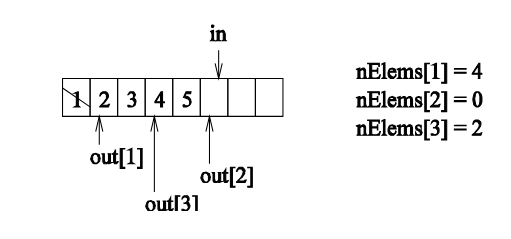
\includegraphics[width=0.5\textwidth]{images/ej79.png}
  \caption{Esquema de interacción entre el productor y los consumidores.}
  \label{fig:ejercicio79}
\end{figure}

\subsection{Solución versión Profesor}

\begin{lstlisting}[style=customcpp, caption={Pseudocódigo del proceso Buffer}]
  process Buffer;

  var
    out: array[0..2] of integer; // Punteros de salida para cada consumidor.
    nElems: array[0..2] of integer; // Número de elementos que quedan por consumir para cada consumidor.
    
    B: integer; // Tamaño del buffer.
    buf: array[0..B-1]; // Buffer acotado de tamaño B.
    begin
    select for i:=0 to 2 do 
      
      when nElemens[i] != 0 do // Si el consumidor i tiene elementos por consumir...
        send (buf[out[i]], consumidor[i]); // Envía el elemento al consumidor i.
        out[i] + 1 mod B; // Actualiza el puntero de salida del consumidor i.
        nElemens[i] = nElemens[i]-1; // Decrementa el número de elementos por consumir del consumidor i.
      end do
      
      when nElemens[0] != B or nElemens[1] != B or nElemens[2] != B do // Si el buffer no está lleno para algún consumidor...
        receive(dato, productor); // Recibe un dato del productor.
        bufer[i] = dato; // Almacena el dato en el buffer.
        for j:=0 to 2 do
          nElemens[j] = nElemens[j] + 1; // Incrementa el número de elementos por consumir para cada consumidor.
        end do
      end do
    end select
  end
\end{lstlisting}

\subsubsection*{Explicación del código del proceso Buffer}

El proceso Buffer se encarga de gestionar la interacción entre un productor y tres consumidores que comparten un buffer acotado de tamaño \( B \). Cada elemento depositado por el productor debe ser retirado por todos los consumidores para ser eliminado del buffer.
La idea general del código es mantener un buffer acotado de tamaño \( B \) donde el productor puede depositar elementos y los consumidores pueden retirarlos. Cada consumidor tiene su propio puntero de salida y contador de elementos por consumir. El proceso Buffer asegura que cada elemento depositado por el productor sea retirado por todos los consumidores antes de ser eliminado del buffer. Además, se asegura de que el buffer no se llene completamente para ningún consumidor y que los consumidores retiren los elementos en el mismo orden en el que fueron depositados.





\subsection{Solución versión Propia}

\begin{lstlisting}[style=customcpp, caption={Pseudocódigo del proceso Buffer}]
  process Buffer;

  var
    out: array[0..2] of integer; // Punteros de salida para cada consumidor.
    nElems: array[0..2] of integer; // Número de elementos que quedan por consumir para cada consumidor.
    
    B: integer; // Tamaño del buffer.
    buf: array[0..B-1]; // Buffer acotado de tamaño B.
    ocupadas: integer := 0; // Número de celdas ocupadas en el buffer.
    begin
    select for i:=0 to 2 do 

      when nElemens[i] != 0 do // Si el consumidor i tiene elementos por consumir...
        send (buf[out[i]], consumidor[i]); // Envía el elemento al consumidor i.
        out[i] + 1 mod B; // Actualiza el puntero de salida del consumidor i.
        nElemens[i] = nElemens[i]-1; // Decrementa el número de elementos por consumir del consumidor i.
      end do
      
      when nElemens[0] != B or nElemens[1] != B or nElemens[2] != B do // Si el buffer no está lleno para algún consumidor...
        receive(dato, productor); // Recibe un dato del productor.
        bufer[ocupadas] = dato; // Almacena el dato en el buffer.
        ocupadas++;
        for j:=0 to 2 do
          nElemens[j] = nElemens[j] + 1; // Incrementa el número de elementos por consumir para cada consumidor.
        end do
      end do

    end select
  end
\end{lstlisting}

\subsubsection*{Explicación del código del proceso Buffer}

El proceso Buffer se encarga de gestionar la interacción entre un productor y tres consumidores que comparten un buffer acotado de tamaño \( B \). Cada elemento depositado por el productor debe ser retirado por todos los consumidores para ser eliminado del buffer.
La idea general del código es mantener un buffer acotado de tamaño \( B \) donde el productor puede depositar elementos y los consumidores pueden retirarlos. Cada consumidor tiene su propio puntero de salida y contador de elementos por consumir. El proceso Buffer asegura que cada elemento depositado por el productor sea retirado por todos los consumidores antes de ser eliminado del buffer. Además, se asegura de que el buffer no se llene completamente para ningún consumidor y que los consumidores retiren los elementos en el mismo orden en el que fueron depositados.


Ahora añadimos los procesos Productor y Consumidor:

\begin{lstlisting}[language=C++]
  process Productor[ i : 0..2 ] ;
  var dato : integer ;
  begin
    while true do begin
      dato := Producir();
      send( dato, Buffer );
    end
  end
  
  process Consumidor ;
  begin
    while true do begin
      receive ( dato, Buffer );
      Consumir( dato );
    end
  end

\end{lstlisting}

    




\section{Ejercicio 80}

\subsection{Enunciado}

\subsection*{Implementación de los procesos Salvajes y Cocinero}

Una tribu de antropófagos comparte una olla en la que caben \(M\) misioneros. Cuando algún salvaje quiere comer, se sirve directamente de la olla, a no ser que ésta esté vacía. Si la olla está vacía, el salvaje despertará al cocinero y esperará a que éste haya rellenado la olla con otros \(M\) misioneros.

\begin{lstlisting}[style=customcpp]
process Salvaje[ i : 0..2 ] ;
begin
    var peticion : integer := ... ;
    begin
        while true do begin
            // esperar a servirse un misionero
            s_send( peticion, Olla );
            // comer:
            Comer();
        end
    end
end

process Cocinero ;
begin 
    while true do begin
        // dormir esperando solicitud para llenar
        // ...
        // confirmar que se ha rellenado la olla
        // ...
    end
end
\end{lstlisting}

Implementar los procesos salvajes y cocinero usando paso de mensajes, utilizando un proceso Olla que incluye una construcción de espera selectiva que sirve peticiones de los salvajes y el cocinero para mantener la sincronización requerida, teniendo en cuenta que:

\begin{itemize}
    \item La solución no debe producir interbloqueo.
    \item Los salvajes podrán comer siempre que haya comida en la olla.
    \item Solamente se despertará al cocinero cuando la olla esté vacía.
\end{itemize}

\subsection{Solución}

\begin{lstlisting}[style=customcpp, caption={Pseudocódigo del proceso Olla}]
process Olla;

var
    comida: integer := 0; // Cantidad de comida disponible en la olla.
    capacidad: integer := M; // Capacidad máxima de la olla.
    peticiones: queue of integer; // Cola para gestionar las peticiones de los salvajes.

begin
    select
        when not peticiones.empty() and comida > 0 do
            // Atender a un salvaje que quiere comer
            salvaje := peticiones.pop();
            comida := comida - 1;
            send("comer", salvaje);
        end

        when comida = 0 do
            // Solicitar al cocinero que rellene la olla
            send("rellenar", cocinero);
            receive("rellenado", cocinero);
            comida := capacidad;
        end
    end select
end
\end{lstlisting}

\begin{lstlisting}[style=customcpp, caption={Pseudocódigo del proceso Salvaje}]
process Salvaje[i: 0..N-1];

begin
    while true do
        // Solicitar comida a la olla
        send(i, Olla);
        receive("comer", Olla);
        Comer();
    end
end
\end{lstlisting}

\begin{lstlisting}[style=customcpp, caption={Pseudocódigo del proceso Cocinero}]
process Cocinero;

begin
    while true do
        // Esperar solicitud para rellenar la olla
        receive("rellenar", Olla);
        // Rellenar la olla
        Rellenar();
        send("rellenado", Olla);
    end
end
\end{lstlisting}

Esta solución asegura:

\begin{itemize}
    \item Sincronización adecuada entre salvajes y cocinero mediante paso de mensajes.
    \item Los salvajes pueden comer siempre que haya comida en la olla.
    \item El cocinero solo se despierta cuando la olla esté vacía.
    \item Evita el interbloqueo utilizando una cola para gestionar las peticiones de los salvajes.
\end{itemize}



\section{Ejercicio 81}

\subsection{Enunciado}

Considerar un conjunto de $N$ procesos, $P[i]$, $(i = 0, \dots, N - 1)$ que se pasan mensajes cada uno al siguiente (y el primero al último), en forma de anillo. Cada proceso tiene un valor local almacenado en su variable local \texttt{mi\_valor}. Deseamos calcular la suma de los valores locales almacenados por los procesos de acuerdo con el algoritmo que se expone a continuación. 

\begin{figure}[H]
  \centering
  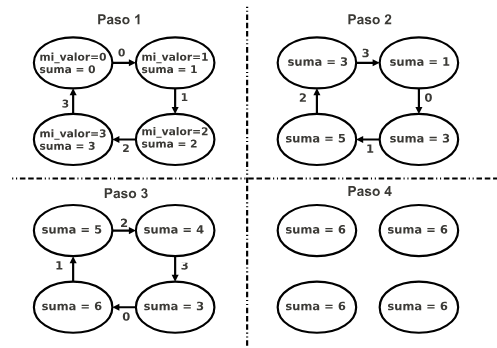
\includegraphics[width=0.9\textwidth]{images/ej81.png}
  \caption{Esquema de interacción entre los procesos.}
  \label{fig:ejercicio81}
\end{figure}


Los procesos realizan una serie de iteraciones para hacer circular sus valores locales por el anillo. En la primera iteración, cada proceso envía su valor local al siguiente proceso del anillo, al mismo tiempo que recibe del proceso anterior el valor local de éste. A continuación acumula la suma de su valor local y el recibido desde el proceso anterior. En las siguientes iteraciones, cada proceso envía al siguiente proceso siguiente el valor recibido en la anterior iteración, al mismo tiempo que recibe del proceso anterior un nuevo valor. Después acumula la suma. Tras un total de $N - 1$ iteraciones, cada proceso conocerá la suma de todos los valores locales de los procesos.



Dar una descripción en pseudocódigo de los procesos siguiendo un estilo SPMD y usando operaciones de envío y recepción síncronas:

\begin{lstlisting}[style=customcpp]
process P[ i : 0..N-1 ] ;
var mi_valor : integer := ... ; // valor arbitrario (== i en la figura, por ejemplo)
    suma : integer := mi_valor ; // suma inicializada a mi_valor
begin
    for j := 0 to N-1 do begin
        ...
    end
end
\end{lstlisting}


\subsection{Solución}

En este caso se afirma que se debe de seguir un estilo SPMD (Single Program Multiple Data), lo que significa que todos los procesos ejecutan el mismo código, pero con datos diferentes. En este caso, cada proceso $P[i]$ tiene un valor local $mi\_valor$ que se suma a la suma total.

\begin{lstlisting}[style=customcpp]
  process P[ i : 0..N-1 ] ;
  var mi_valor : integer := i ; // valor arbitrario (== i en la figura, por ejemplo)
      suma : integer := mi_valor ; // suma inicializada a mi_valor
  begin
      for j := 0 to N-1 do begin
          send( mi_valor, P[ (i + 1) mod N ] );
          receive( valor_recibido, P[ (i - 1 + N) mod N ] );
          suma := suma + valor_recibido;
          mi_valor := valor_recibido; 
      end
  end
\end{lstlisting}

\section{Ejercicio 82}

\subsection{Enunciado}

Considerar un estanco en el que hay tres fumadores y un estanquero. Cada fumador continuamente lía un cigarro y se lo fuma. Para liar un cigarro, el fumador necesita tres ingredientes: tabaco, papel y cerillas. Uno de los fumadores tiene solamente papel, otro tiene solamente tabaco, y el otro tiene solamente cerillas. El estanquero tiene una cantidad infinita de los tres ingredientes.

El estanquero coloca aleatoriamente dos ingredientes diferentes de los tres que se necesitan para hacer un cigarro, desbloquea al fumador que tiene el tercer ingrediente y después se bloquea. El fumador seleccionado se puede obtener fácilmente mediante una función \texttt{genera\_ingredientes} que devuelve el índice (0, 1, ó 2) del fumador escogido.

El fumador desbloqueado toma los dos ingredientes del mostrador, desbloqueando al estanquero, lía un cigarro y fuma durante un tiempo. El estanquero, una vez desbloqueado, vuelve a poner dos ingredientes aleatorios en el mostrador, y se repite el ciclo.

Describir una solución distribuida que use envío asíncrono seguro y recepción síncrona para este problema usando un proceso Estanquero y tres procesos fumadores Fumador(i) (con $i=0,1$ y $2$).

\begin{lstlisting}[style=customcpp]
process Estanquero ;
begin
    while true do begin
        // El estanquero coloca dos ingredientes aleatorios en el mostrador
        // y desbloquea al fumador que tiene el tercer ingrediente
        ...
    end
end

process Fumador[ i : 0..2 ] ;
begin
    while true do begin
        // El fumador espera hasta que sea desbloqueado
        // Toma los dos ingredientes del mostrador, lía un cigarro y fuma
        ...
    end
end
\end{lstlisting}

\subsection{Solución}

\textit{Usando envío asíncrono seguro y recepción síncrona.} Para ello debemos de usar MPI\_Isend y MPI\_Recv.

\begin{lstlisting}[style=customcpp]
  process Estanquero ;
  begin
      while true do begin
          // El estanquero coloca dos ingredientes aleatorios en el mostrador
          int ingrediente1, ingrediente2;
          ingrediente1 = generarIngrediente();
          do{
              ingrediente2 = generarIngrediente();
          }
          while(ingrediente1 == ingrediente2);
          // y desbloquea al fumador que tiene el tercer ingrediente
          MPI_Isend(ingrediente1, 1, MPI_INT, Fumador[3 - ingrediente1 - ingrediente2], 0, MPI_COMM_WORLD);
          MPI_Isend(ingrediente2, 1, MPI_INT, Fumador[3 - ingrediente1 - ingrediente2], 0, MPI_COMM_WORLD);
      end
  end
  
  process Fumador[ i : 0..2 ] ;
  begin
      while true do begin
          // El fumador espera hasta que sea desbloqueado
          int ingrediente1, ingrediente2;
          MPI_Recv(ingrediente1, 1, MPI_INT, Estanquero, 0, MPI_COMM_WORLD, MPI_STATUS_IGNORE);
          MPI_Recv(ingrediente2, 1, MPI_INT, Estanquero, 0, MPI_COMM_WORLD, MPI_STATUS_IGNORE);
          // Toma los dos ingredientes del mostrador, lía un cigarro y fuma
          LiarCigarro();
          Fumar();
      end
  end
\end{lstlisting}

\textit{En este caso no hemos usado select porque no es necesario, ya que el estanquero siempre coloca los ingredientes y los fumadores siempre esperan a recibirlos.}

\subsection{Solución 2}

\textit{Usando \texttt{select} para modelar la interacción entre el estanquero y los fumadores.}

En esta solución, utilizamos el mecanismo de \texttt{select}, que permite manejar múltiples condiciones de sincronización para coordinar a los procesos. A continuación, se presenta el código:

\begin{lstlisting}[style=customcpp]
process Estanquero ;
begin
    while true do begin
        // El estanquero coloca dos ingredientes aleatorios en el mostrador
        int ingrediente1, ingrediente2;
        ingrediente1 = generarIngrediente();
        do {
            ingrediente2 = generarIngrediente();
        }
        while (ingrediente1 == ingrediente2);
        
        // Selecciona al fumador que necesita el tercer ingrediente
        int fumador = 3 - ingrediente1 - ingrediente2;
        enviar(ingrediente1, fumador);
        enviar(ingrediente2, fumador);
    end
end

process Fumador[ i : 0..2 ] ;
begin
    while true do begin
        select 
            when recibir(ingrediente1, Estanquero) and  recibir(ingrediente2, Estanquero) do begin
                // Toma los dos ingredientes del mostrador
                LiarCigarro();
                Fumar();
        end // select
    end
end
\end{lstlisting}

En esta implementación:
\begin{itemize}
    \item El \texttt{process Estanquero} utiliza una lógica similar para seleccionar aleatoriamente los ingredientes y desbloquear al fumador correspondiente.
    \item El \texttt{process Fumador} usa \texttt{select} para esperar a recibir los ingredientes necesarios. Este enfoque permite que el fumador gestione la recepción de ambos ingredientes de manera no bloqueante, mejorando la sincronización en sistemas distribuidos.
\end{itemize}

Ambas soluciones son válidas para el problema planteado, pero la elección entre ellas puede depender de las restricciones de diseño y el entorno de implementación.


\section{Ejercicio 83}

\subsection{Enunciado}

En un sistema distribuido, un gran número de procesos clientes usa frecuentemente un determinado recurso y se desea que puedan usarlo simultáneamente el máximo número de procesos. Para ello, los clientes envían peticiones a un proceso controlador para usar el recurso y esperan respuesta para poder usarlo (véase el código de los procesos clientes). Cuando un cliente termina de usar el recurso, envía una solicitud para dejar de usarlo y espera respuesta del Controlador. El proceso controlador se encarga de asegurar la sincronización adecuada imponiendo una única restricción por razones supersticiosas: nunca habrá 13 procesos exactamente usando el recurso al mismo tiempo.

\begin{lstlisting}[style=customcpp]
process Cli[ i : 0....n ] ;
var pet_usar : integer := +1 ;
    pet_liberar : integer := -1 ;
    permiso : integer := ... ;
begin
    while true do begin
        send( pet_usar, Controlador );
        receive( permiso, Controlador );
        Usar_recurso( );
        send( pet_liberar, Controlador );
        receive( permiso, Controlador );
    end
end
\end{lstlisting}

\begin{lstlisting}[style=customcpp]
process Controlador ;
begin
    while true do begin
        select
            ...
        end
end
\end{lstlisting}

Describir en pseudocódigo el comportamiento del proceso controlador, utilizando una orden de espera selectiva que permita implementar la sincronización requerida entre los procesos. Es posible utilizar una sentencia del tipo select for i=... to ... para especificar diferentes ramas de una sentencia selectiva que comparten el mismo código dependiente del valor de un índice i.

\subsection{Solución}

\begin{lstlisting}[style=customcpp]
  
  process Controlador ;
  var contador: integer;
  begin
      while true do begin
          select
            for i:= 0 to n do 

              when receive(pet_usar,Cli[i]) do 
                if contador < 13 then 
                  send(permiso,Cli[i]);
                  contador := contador + 1;
                end if
              end do  

              when receive(pet_liberar,Cli[i]) do 
                send(permiso,Cli[i]);
                contador := contador - 1;
              end do
          
          end select
      end 
  end

\end{lstlisting}

\subsubsection*{Lógica de la solución}

En este caso se ha pensado la solución de manera simple. Se trata de un controlador que recibe peticiones de los clientes para usar un recurso. Si el contador de procesos que están usando el recurso es menor que 13, el controlador envía un permiso al cliente para que pueda usar el recurso. Cuando un cliente termina de usar el recurso, envía una petición para liberarlo y el controlador disminuye el contador. De esta forma, se asegura que nunca haya exactamente 13 procesos usando el recurso al mismo tiempo. Es impotante \textbf{uso del if} para asegurarnos de que solo se usan los 13 procesos a la vez, y debemos de asegurarnos de que actualizamos de manera correcta la variable contador.

\section{Ejercicio 84}

\subsection{Enunciado}

En un sistema distribuido, tres procesos Productor se comunican con un proceso Impresor que se encarga de ir imprimiendo en pantalla una cadena con los datos generados por los procesos productores. Cada proceso productor (\texttt{Productor[i]} con \(i = 0, 1, 2\)) genera continuamente el correspondiente entero \(i\), y lo envía al proceso Impresor.

El proceso Impresor se encarga de ir recibiendo los datos generados por los productores y los imprime por pantalla (usando el procedimiento \texttt{imprime(entero)}) generando una cadena de dígitos en la salida. No obstante, los procesos se han de sincronizar adecuadamente para que la impresión por pantalla cumpla las siguientes restricciones:

\begin{itemize}
    \item Los dígitos 0 y 1 deben aceptarse por el impresor de forma alterna. Es decir, si se acepta un 0 no podrá volver a aceptarse un 0 hasta que se haya aceptado un 1, y viceversa, si se acepta un 1 no podrá volver a aceptarse un 1 hasta que se haya aceptado un 0.
    \item El número total de dígitos 0 o 1 aceptados en un instante no puede superar el doble de número de dígitos 2 ya aceptados en dicho instante.
\end{itemize}

Cuando un productor envía un dígito que no se puede aceptar por el impresor, el productor quedará bloqueado esperando completar el \texttt{s\_send}. El pseudocódigo de los procesos productores (\texttt{Productor}) se muestra a continuación, asumiendo que se usan operaciones bloqueantes no buferizadas (síncronas):

\begin{lstlisting}[style=customcpp]
process Productor[ i : 0,1,2 ]
while true do begin
    s_send( i, Impresor ) ;
end
\end{lstlisting}

\begin{lstlisting}[style=customcpp, caption={Pseudocódigo del proceso Impresor}]
process Impresor
  var
      .....
    begin
      while true do begin
        select
          .....
        end
      end
    end
\end{lstlisting}


\subsection{Solución}

% \begin{lstlisting}[style=customcpp]
% process Impresor
% var
%     contador_0_1 : integer := 0 ;
%     contador_2 : integer := 0 ;
%     turno : integer := 0 ; // 0: turno para aceptar 0, 1: turno para aceptar 1
% begin
%     while true do begin
%         select
%             when receive(dato, Productor[0]) do
%                 if (dato == 0 and turno == 0 and contador_0_1 < 2 * contador_2) then
%                     imprime(dato);
%                     contador_0_1 := contador_0_1 + 1;
%                     turno := 1;
%                 else if (dato == 1 and turno == 1 and contador_0_1 < 2 * contador_2) then
%                     imprime(dato);
%                     contador_0_1 := contador_0_1 + 1;
%                     turno := 0;
%                 else if (dato == 2) then
%                     imprime(dato);
%                     contador_2 := contador_2 + 1;
%                 end if;
%             end when
%             when receive(dato, Productor[1]) do
%                 if (dato == 0 and turno == 0 and contador_0_1 < 2 * contador_2) then
%                     imprime(dato);
%                     contador_0_1 := contador_0_1 + 1;
%                     turno := 1;
%                 else if (dato == 1 and turno == 1 and contador_0_1 < 2 * contador_2) then
%                     imprime(dato);
%                     contador_0_1 := contador_0_1 + 1;
%                     turno := 0;
%                 else if (dato == 2) then
%                     imprime(dato);
%                     contador_2 := contador_2 + 1;
%                 end if;
%             end when
%             when receive(dato, Productor[2]) do
%                 if (dato == 0 and turno == 0 and contador_0_1 < 2 * contador_2) then
%                     imprime(dato);
%                     contador_0_1 := contador_0_1 + 1;
%                     turno := 1;
%                 else if (dato == 1 and turno == 1 and contador_0_1 < 2 * contador_2) then
%                     imprime(dato);
%                     contador_0_1 := contador_0_1 + 1;
%                     turno := 0;
%                 else if (dato == 2) then
%                     imprime(dato);
%                     contador_2 := contador_2 + 1;
%                 end if;
%             end when
%         end select
%     end
% end
% \end{lstlisting}

\begin{lstlisting}[style=customcpp]
  process Impresor
  var
      contador_0_1 : integer := 0 ;
      contador_2 : integer := 0 ;
      turno : integer := 0 ; // 0: turno para aceptar 0, 1: turno para aceptar 1
  begin
      while true do begin
          select
            for i:= 0 to 2
              when receive(dato, Productor[i]) do
                  if (dato == 0 and turno == 0 and contador_0_1 < 2 * contador_2) then
                      imprime(dato);
                      contador_0_1 := contador_0_1 + 1;
                      turno := 1;
                  else if (dato == 1 and turno == 1 and contador_0_1 < 2 * contador_2) then
                      imprime(dato);
                      contador_0_1 := contador_0_1 + 1;
                      turno := 0;
                  else if (dato == 2) then
                      imprime(dato);
                      contador_2 := contador_2 + 1;
                  end if;
              end when
          end select
      end
  end
  \end{lstlisting}


\subsubsection*{Lógica de la solución}

En este código del proceso \texttt{Impresor}, se maneja la sincronización entre los productores y el impresor usando un \texttt{select}, y además diseñandolo la solución usando la opción for para hacer más simple el código. Para cada productor, se controla la aceptación de los dígitos 0, 1 y 2, con las restricciones mencionadas en el enunciado. El proceso acepta un dígito según las condiciones del turno (alternancia entre 0 y 1) y el límite sobre el número de dígitos 0 y 1 que pueden aceptarse en comparación con los dígitos 2.


\section{Ejercicio 85}

\subsection{Enunciado}

En un sistema distribuido hay un vector de \(n\) procesos iguales que envían con \texttt{send} (en un bucle infinito) valores enteros a un proceso receptor, que los imprime. Si en algún momento no hay ningún mensaje pendiente de recibir en el receptor, este proceso debe imprimir "no hay mensajes, duermo"; después de bloquearse durante 10 segundos (con \texttt{sleep\_for(10)}), antes de volver a comprobar si hay mensajes (esto podría hacerse para ahorrar energía, ya que el procesamiento de mensajes se hace en ráfagas separadas por 10 segundos).

Este problema no se puede solucionar usando \texttt{receive} o \texttt{i\_receive}. Indica a qué se debe esto. Sin embargo, sí se puede hacer con \texttt{select}. Diseña una solución a este problema con \texttt{select}:

\begin{lstlisting}[style=customcpp]
process Emisor[ i : 1..n ]
var dato : integer ;
begin
    while true do begin
        dato := Producir() ;
        send( dato, Receptor );
    end
end
\end{lstlisting}

\begin{lstlisting}[style=customcpp]
process Receptor()
var dato : integer ;
begin
    while true do
        ......
end
\end{lstlisting}


\subsection{Solución}

Para resolver este problema, utilizamos un enfoque basado en \texttt{select}, ya que ni \texttt{receive} ni \texttt{i\_receive} permiten detectar si no hay mensajes pendientes de forma directa. Esto se debe a que:

\begin{itemize}
    \item \texttt{receive} es una operación bloqueante que espera hasta que haya un mensaje disponible, impidiendo que podamos comprobar si no hay mensajes sin bloquear el proceso.
    \item \texttt{i\_receive} es una operación no bloqueante, pero simplemente devuelve un indicador de éxito o fallo y no permite implementar un mecanismo de espera como el solicitado.
\end{itemize}

Con \texttt{select}, podemos implementar un mecanismo de espera que permita al proceso receptor manejar mensajes cuando estén disponibles, o ejecutar una acción alternativa (como imprimir "no hay mensajes, duermo") si no hay mensajes. La solución se describe a continuación:

\begin{lstlisting}[style=customcpp]
process Emisor[ i : 1..n ]
var dato : integer ;
begin
    while true do begin
        dato := Producir(); // Generar un nuevo dato
        send(dato, Receptor); // Enviar el dato al Receptor
    end
end
\end{lstlisting}

\begin{lstlisting}[style=customcpp]
process Receptor()
var dato : integer ;
begin
    while true do begin
        select
            when receive(dato, Emisor[1..n]) do // Si hay mensajes
                imprime(dato); // Imprimir el mensaje recibido
            else // Si no hay mensajes pendientes
                imprime("no hay mensajes, duermo");
                sleep_for(10); // Bloquear durante 10 segundos
        end select
    end
end
\end{lstlisting}

\subsubsection*{\textbf{Explicación de la solución}}

\textbf{1. Emisor:}  
Cada proceso \texttt{Emisor[i]} produce un valor entero con la función \texttt{Producir()} y lo envía al \texttt{Receptor} utilizando la operación \texttt{send}. Este proceso se ejecuta en un bucle infinito.

\textbf{2. Receptor:}  
El proceso \texttt{Receptor} implementa un bucle infinito que realiza las siguientes acciones:
\begin{itemize}
  \item Usa una sentencia \texttt{select} para manejar dos escenarios:
  \begin{itemize}
    \item Si hay mensajes disponibles, el receptor los consume con \texttt{receive} y los imprime utilizando \texttt{imprime(dato)}.
    \item Si no hay mensajes pendientes (gracias al \texttt{else} del \texttt{select}), el receptor imprime ``no hay mensajes, duermo'' y entra en un estado de espera por 10 segundos usando \texttt{sleep\_for(10)}.
  \end{itemize}
\end{itemize}
\textbf{3. Uso de \texttt{select}:}  
La operación \texttt{select} permite al proceso \texttt{Receptor} manejar la recepción de mensajes de múltiples emisores (\texttt{Emisor[1..n]}), así como realizar una acción alternativa (\texttt{else}) cuando no hay mensajes pendientes.

\subsubsection*{\textbf{Respuesta a las preguntas planteadas}}

\textbf{1. ¿Por qué no se puede solucionar el problema con \texttt{receive} o \texttt{i\_receive}?}  
\begin{itemize}
  \item \texttt{receive} es bloqueante, lo que significa que el receptor esperará indefinidamente hasta que llegue un mensaje, impidiendo detectar que no hay mensajes.
  \item \texttt{i\_receive} no es bloqueante, pero solo devuelve un indicador de éxito o fallo. No proporciona un mecanismo para realizar acciones alternativas cuando no hay mensajes pendientes, como el que se implementa con \texttt{select}.
\end{itemize}

\textbf{2. ¿Por qué es útil \texttt{select}?}  
\begin{itemize}
  \item \texttt{select} permite manejar múltiples condiciones de recepción de mensajes y, además, proporciona un mecanismo \texttt{else} para definir acciones alternativas cuando ninguna condición se cumple. Esto es crucial para implementar el comportamiento del receptor cuando no hay mensajes.
\end{itemize}

Con esta implementación, se garantiza que el \texttt{Receptor} cumpla con las especificaciones planteadas: procesar mensajes cuando estén disponibles o entrar en un estado de espera eficiente si no hay mensajes.



\section{Ejercicio 86}
\subsection{Enunciado}

En un sistema tenemos \textbf{N procesos emisores} que envían de forma segura un único mensaje cada uno de ellos a un proceso receptor. El mensaje contiene un entero con el número del proceso emisor. El proceso receptor debe imprimir el número del proceso emisor que inició el envío en primer lugar. Dicho emisor debe terminar, y el resto quedarse bloqueados:

\begin{lstlisting}[style=customcpp]
process Emisor[ i : 1.. N ]
begin
    s_send(i, Receptor);
end

process Receptor ;
var ganador : integer ;
begin
    // calcular ganador
    ....
    ....
    print "El primer envío lo ha realizado: ....", ganador;
end
\end{lstlisting}

Para cada uno de los siguientes casos, describir razonadamente si es posible diseñar una solución a este problema o no lo es. En caso afirmativo, escribe una posible solución:

\begin{enumerate}
    \item[(a)] El proceso receptor usa exclusivamente recepción mediante una o varias llamadas a \texttt{receive}.
    \item[(b)] El proceso receptor usa exclusivamente recepción mediante una o varias llamadas a \texttt{i\_receive}.
    \item[(c)] El proceso receptor usa exclusivamente recepción mediante una o varias instrucciones \texttt{select}.
\end{enumerate}

\subsection{Solución}

A continuación, se analiza cada uno de los casos planteados y se proporciona una solución cuando es posible:
\begin{enumerate}[label=\alph*)]

\item \textbf{ Recepción exclusivamente mediante \texttt{receive}:}

Usar \texttt{receive} garantiza que el proceso receptor obtiene un mensaje completo antes de procesarlo, lo que permite determinar cuál fue el primer emisor. Sin embargo, \texttt{receive} no tiene orden garantizado cuando varios emisores envían simultáneamente. Para garantizar que se identifica correctamente al primer emisor, los mensajes deben llegar en el orden en que fueron enviados.

\textbf{Solución:}

\begin{lstlisting}[style=customcpp]
process Receptor ;
var ganador : integer ;
    recibido : integer ;
    encontrado : boolean := false ;
begin
    while not encontrado do begin
        receive(recibido, *);  // Recibir de cualquier emisor
        if not encontrado then begin
            ganador := recibido;  // El primer mensaje recibido
            encontrado := true;
            print "El primer envío lo ha realizado: ", ganador;
        end
    end
end
\end{lstlisting}

En esta solución:
\begin{itemize}
    \item El receptor procesa el primer mensaje recibido y almacena el identificador del emisor como \texttt{ganador}.
    \item Los demás emisores quedan bloqueados porque el receptor no solicita más mensajes.
\end{itemize}

\item \textbf{ Recepción exclusivamente mediante \texttt{i\_receive}:}

La operación \texttt{i\_receive} permite verificar si un mensaje está disponible sin bloquearse. Sin embargo, \texttt{i\_receive} no garantiza un orden, por lo que sería necesario iterar constantemente para determinar el primer emisor. Esto puede generar comportamiento indeterminado, ya que \texttt{i\_receive} solo indica disponibilidad y no un orden temporal.

\textbf{Conclusión:} No es posible garantizar que el primer mensaje sea procesado correctamente usando solo \texttt{i\_receive}.

\item \textbf{ Recepción exclusivamente mediante \texttt{select}:}

La instrucción \texttt{select} permite manejar múltiples canales de recepción simultáneamente. Esto asegura que el receptor atienda el primer mensaje recibido en cualquiera de los canales, determinando así correctamente al primer emisor.

\textbf{Solución:}

\begin{lstlisting}[style=customcpp]
process Receptor ;
var ganador : integer ;
    recibido : integer ;
    encontrado : boolean := false ;
begin
    while not encontrado do begin
        select
            for i := 1 to N do
                when receive(recibido, Emisor[i]) do begin
                    ganador := recibido;  // El primer mensaje recibido
                    encontrado := true;
                    print "El primer envío lo ha realizado: ", ganador;
                end
            end for
        end select
    end
end
\end{lstlisting}

En esta solución:
\begin{itemize}
    \item El receptor utiliza \texttt{select} para atender al primer mensaje recibido desde cualquier emisor.
    \item El bucle asegura que se identifica al emisor más rápido, y se imprime su número.
    \item Los emisores restantes quedan bloqueados, ya que no se procesan más mensajes después de encontrar al ganador.
\end{itemize}

\end{enumerate}

\begin{tcolorbox}[colback=gray!5!white,colframe=gray!75!black,title=\textbf{Resumen:}]

  \begin{enumerate}[label=\alph*)]
    \item Es posible resolver el problema usando \texttt{receive}, y la solución es viable.
    \item No es posible garantizar una solución con \texttt{i\_receive}, debido a la falta de orden y bloqueo.
    \item Es posible resolver el problema con \texttt{select}, y la solución es eficiente y correcta.
  \end{enumerate}
\end{tcolorbox}




\section{Ejercicio 87}

\subsection{Enunciado}

Supongamos que tenemos \textbf{N} procesos concurrentes semejantes:

\begin{lstlisting}[style=customcpp]
process P[ i : 1..N ] ;
    ....
  begin
    ....
  end
\end{lstlisting}

Cada proceso produce \textbf{N-1 caracteres} (con \texttt{N-1} llamadas a la función \texttt{ProduceCaracter}) y envía cada carácter a los otros \texttt{N-1} procesos. Además, cada proceso debe imprimir todos los caracteres recibidos de los otros procesos (el orden en el que se escriben es indiferente).

\begin{itemize}
    \item \textbf{Describe razonadamente si es o no posible hacer esto usando exclusivamente \texttt{s\_send} para los envíos.} En caso afirmativo, escribe una solución.
    \item \textbf{Escribe una solución usando \texttt{send} y \texttt{receive}.}
\end{itemize}

\subsection{Solución}

\begin{itemize} 

\item \textbf{1. Análisis del uso exclusivo de \texttt{s\_send}:}

El uso exclusivo de \texttt{s\_send} (envío sin búfer y bloqueante) puede causar problemas de interbloqueo en este escenario. Dado que \texttt{s\_send} requiere que el receptor esté listo para recibir el mensaje en el momento del envío, si todos los procesos están intentando enviar al mismo tiempo y ninguno está recibiendo, el sistema se bloqueará.\\

Por lo tanto, \textbf{no es posible implementar esta solución utilizando exclusivamente \texttt{s\_send}} debido a la naturaleza de la operación bloqueante.\\


\item  \textbf{2. Solución utilizando \texttt{send} y \texttt{receive}:}

Para resolver este problema, se utiliza una combinación de \texttt{send} y \texttt{receive}, asegurando que cada proceso envíe sus caracteres a los demás procesos y, al mismo tiempo, reciba los caracteres enviados por otros procesos.\\

\begin{lstlisting}[style=customcpp]
process P[ i : 1..N ] ;
var
    caract : char ;       // Carácter producido
    recibido : char ;     // Carácter recibido
begin
    // Enviar N-1 caracteres a los otros procesos
    for j := 1 to N do
        if j != i then begin
            caract := ProduceCaracter(); // Produce un carácter
            send(caract, P[j]);          // Enviar al proceso P[j]
        end
    end

    // Recibir N-1 caracteres de los otros procesos
    for j := 1 to N do
        if j != i then begin
            receive(recibido, P[j]);      // Recibir de proceso P[j]
            imprime(recibido);           // Imprimir el carácter recibido
        end
    end
end
\end{lstlisting}

\textbf{Explicación de la solución:}

\begin{itemize}
    \item Cada proceso \texttt{P[i]} realiza dos bucles:
    \begin{itemize}
        \item En el primer bucle, genera \texttt{N-1} caracteres con la función \texttt{ProduceCaracter} y los envía a los otros \texttt{N-1} procesos utilizando \texttt{send}.
        \item En el segundo bucle, recibe los caracteres enviados por los otros \texttt{N-1} procesos utilizando \texttt{receive} y los imprime.
    \end{itemize}
    \item Para evitar enviar mensajes a sí mismo, se incluye la condición \texttt{if j != i}.
    \item El uso de \texttt{send} y \texttt{receive} permite que los procesos se sincronicen correctamente sin riesgo de interbloqueo, ya que las operaciones de recepción permiten manejar los mensajes enviados.
\end{itemize}

\end{itemize}






\section{Ejercicio 88}

\subsection{Enunciado}

Escribe una nueva solución al problema anterior en la cual se garantice que el orden en el que se imprimen los caracteres es el mismo orden en el que se inician los envíos de dichos caracteres. 

\textbf{Pista:} usa \texttt{select} para recibir.

\subsection{Solución}

Para garantizar que los caracteres se impriman en el mismo orden en el que se inician los envíos, utilizamos la instrucción \texttt{select} en el proceso receptor. Esto permite gestionar de manera ordenada la recepción de los caracteres basándose en el orden de llegada de los mensajes.

\begin{lstlisting}[style=customcpp]
process P[ i : 1..N ] ;
var
    caract : char ;       // Carácter producido
begin
    // Enviar N-1 caracteres a los otros procesos
    for j := 1 to N do
        if j != i then begin
            caract := ProduceCaracter(); // Produce un carácter
            send(caract, Receptor);      // Enviar al proceso Receptor
        end
    end
end

process Receptor ;
var
    caract : char ;       // Carácter recibido
    sender : integer ;    // ID del proceso emisor, se supone que se usa en imprime
    recibido[N] : integer := [0, ..., 0]; // Vector de contadores por emisor, se usa como extra
begin
    while true do begin
        select
            for i := 1 to N do
                when receive(caract, P[i]) do begin
                    imprime(caract, sender);        // Imprimir el carácter recibido
                    //imprime(caract);
                    recibido[i] := recibido[i] + 1; // Actualizar contador
                end
            end
        end select
    end
end
\end{lstlisting}

\textbf{Explicación de la solución:}

\begin{itemize}
    \item \textbf{Proceso \texttt{P[i]}:} 
    \begin{itemize}
        \item Cada proceso genera \texttt{N-1} caracteres usando la función \texttt{ProduceCaracter}.
        \item Los caracteres se envían al proceso \texttt{Receptor} mediante \texttt{send}.
    \end{itemize}
    
    \item \textbf{Proceso \texttt{Receptor}:}
    \begin{itemize}
        \item Utiliza una instrucción \texttt{select} para manejar los mensajes recibidos desde los procesos \texttt{P[i]} en orden de llegada.
        \item Cada mensaje contiene el carácter producido por el proceso emisor y su ID (implícito en la recepción).
        \item Los caracteres se imprimen en el orden de recepción, asegurando que se respeta el orden en el que se iniciaron los envíos.
        \item Un vector \texttt{recibido[i]} se utiliza para llevar un conteo del número de caracteres recibidos de cada proceso, si fuera necesario para el análisis.
    \end{itemize}
\end{itemize}







\section{Ejercicio 89}

\subsection{Enunciado}

Supongamos de nuevo el problema anterior en el cual todos los procesos envían a todos. Ahora cada \textbf{item de datos} a producir y transmitir es un \textbf{bloque de bytes} con muchos valores (por ejemplo, es una imagen que puede tener varios megabytes de tamaño). Se dispone del tipo de datos \texttt{TipoBloque} para ello, y el procedimiento \texttt{ProducirBloque}, de forma que si \texttt{b} es una variable de tipo \texttt{TipoBloque}, entonces la llamada a \texttt{ProducirBloque(b)} produce y escribe una secuencia de bytes en \texttt{b}. 

En lugar de imprimir los datos, se deben consumir con una llamada a \texttt{ConsumirBloque(b)}.

\begin{itemize}
    \item Cada proceso se ejecuta en un ordenador, y se garantiza que hay la suficiente memoria en ese ordenador como para contener simultáneamente, al menos, hasta \texttt{N} bloques.
    \item Sin embargo, el sistema de paso de mensajes (SPM) podría no tener memoria suficiente como para contener los \((N - 1)^2\) mensajes en tránsito simultáneos que podría llegar a haber en un momento dado con la solución anterior.
    \item En estas condiciones, si el \textbf{SPM} agota la memoria, debe retrasar los \texttt{send} dejando bloqueados los procesos y, en esas circunstancias, se podría producir \textbf{interbloqueo}.
    \item Para evitarlo, se pueden usar operaciones inseguras de envío, \texttt{i\_send}. 
\end{itemize}

\textbf{Escribe dicha solución, usando como orden de recepción el mismo que en el problema anterior.}




\subsection{Solución}

Para resolver el problema en el que los procesos envían bloques de datos grandes y garantizar que no haya interbloqueo debido a limitaciones de memoria en el sistema de paso de mensajes, utilizamos operaciones inseguras de envío \texttt{i\_send}. Además, aseguramos que los bloques se reciben en el mismo orden en que se inician los envíos mediante el uso de \texttt{select}.

\begin{lstlisting}[style=customcpp]
process P[ i : 1..N ] ;
var
    bloque : TipoBloque;  // Bloque de datos producido
begin
    // Enviar N-1 bloques de datos a los otros procesos
    for j := 1 to N do
        if j != i then begin
            ProducirBloque(bloque);       // Producir un bloque de datos
            i_send(bloque, Receptor);    // Enviar de manera insegura al Receptor
        end
    end
end

process Receptor ;
var
    bloque : TipoBloque;   // Bloque de datos recibido
    sender : integer;      // ID del proceso emisor
    recibido[N] : integer := [0, ..., 0]; // Vector de contadores por emisor
begin
    while true do begin
        select
            for i := 1 to N do
                when receive(bloque, P[i]) do begin
                    ConsumirBloque(bloque);         // Consumir el bloque recibido
                    recibido[i] := recibido[i] + 1; // Actualizar contador
                end
            end
        end select
    end
end
\end{lstlisting}

\textbf{Explicación de la solución:}

\begin{itemize}
    \item \textbf{Proceso \texttt{P[i]}:} 
    \begin{itemize}
        \item Cada proceso genera \texttt{N-1} bloques de datos usando la función \texttt{ProducirBloque}.
        \item Los bloques se envían al proceso \texttt{Receptor} utilizando \texttt{i\_send}, que es una operación de envío no bloqueante.
        \item Esto garantiza que los procesos emisores no se bloqueen entre sí debido a las limitaciones de memoria del sistema de paso de mensajes.
    \end{itemize}

    \item \textbf{Proceso \texttt{Receptor}:}
    \begin{itemize}
        \item Utiliza una instrucción \texttt{select} para manejar los mensajes recibidos desde los procesos \texttt{P[i]} en orden de llegada.
        \item Cada mensaje contiene el bloque de datos producido por el proceso emisor.
        \item Los bloques se consumen inmediatamente con \texttt{ConsumirBloque}, liberando la memoria del sistema de paso de mensajes.
        \item Un vector \texttt{recibido[i]} se utiliza para llevar un conteo del número de bloques recibidos de cada proceso, si fuera necesario para análisis o depuración.
    \end{itemize}
\end{itemize}

\textbf{Garantías de esta solución:}
\begin{itemize}
    \item \textbf{Evita interbloqueos:} El uso de \texttt{i\_send} permite que los procesos emisores no queden bloqueados si el sistema de paso de mensajes agota la memoria.
    \item \textbf{Orden de recepción:} La instrucción \texttt{select} garantiza que los bloques se procesen en el orden en el que llegan al receptor.
    \item \textbf{Consumo eficiente de memoria:} Los bloques se consumen tan pronto como son recibidos, liberando memoria en el sistema de paso de mensajes.
\end{itemize}

\section{Ejercicio 90}

\subsection{Enunciado}

En los tres problemas anteriores, cada proceso va esperando a recibir un ítem de datos de cada uno de los otros procesos, consume dicho ítem, y después pasa a recibir del siguiente emisor (en distintos órdenes). Esto implica que un envío ya iniciado, pero pendiente, no puede completarse hasta que el receptor no haya consumido los anteriores bloques. Es decir, se podría estar consumiendo mucha memoria en el sistema de paso de mensajes (SPM) por mensajes en tránsito pendientes cuya recepción se ve retrasada.

Escribe una solución en la cual cada proceso inicia sus envíos y recepciones y después espera a que se completen todas las recepciones antes de iniciar el primer consumo de un bloque recibido. De esta forma, todos los mensajes pueden transferirse potencialmente de forma simultánea. Se debe intentar que la transmisión y la producción de bloques sean lo más simultáneas posible.

\textbf{Suponer:} 
\begin{itemize}
    \item Cada proceso puede almacenar como mínimo \texttt{2*N} bloques en su memoria local.
    \item El orden de recepción o de consumo de los bloques es indiferente.
\end{itemize}

\subsection{Solución}

Para implementar esta solución, cada proceso realiza los siguientes pasos:
\begin{enumerate}
  \item Produce \texttt{N-1} bloques y los envía a los otros procesos utilizando \texttt{i\_send}.
  \item Recibe \texttt{N-1} bloques utilizando \texttt{receive}, asegurándose de completar todas las recepciones antes de comenzar a consumir los bloques.
  \item Consume los bloques recibidos en cualquier orden.
\end{enumerate}

\begin{lstlisting}[style=customcpp]
process P[ i : 1..N ] ;
var
    bloquesEnviados[N-1] : TipoBloque;  // Bloques producidos para enviar
    bloquesRecibidos[N-1] : TipoBloque; // Bloques recibidos
    j : integer;                        // Iterador
begin
    // Paso 1: Producir y enviar bloques
    for j := 1 to N do
        if j != i then begin
            ProducirBloque(bloquesEnviados[j]); // Producir un bloque
            i_send(bloquesEnviados[j], P[j]);   // Enviar al proceso P[j]
        end
    end

    // Paso 2: Recibir bloques
    for j := 1 to N do
        if j != i then
            receive(bloquesRecibidos[j], P[j]); // Recibir bloque de P[j]
        end
    end

    // Paso 3: Consumir bloques
    for j := 1 to N do
        if j != i then
            ConsumirBloque(bloquesRecibidos[j]); // Consumir bloque recibido
        end
    end
end
\end{lstlisting}

\textbf{Explicación de la solución:}

\begin{itemize}
    \item \textbf{Producción y envío simultáneos:} Cada proceso genera los bloques para los otros \texttt{N-1} procesos de manera concurrente, enviándolos de inmediato mediante \texttt{i\_send}. Esto permite que la producción y la transmisión sean simultáneas y aprovechen al máximo los recursos del sistema.
    \item \textbf{Recepción antes de consumo:} Cada proceso espera a recibir todos los bloques de los otros procesos antes de comenzar a consumirlos. Esto reduce la memoria ocupada en el sistema de paso de mensajes, ya que los mensajes en tránsito se procesan rápidamente.
    \item \textbf{Orden indiferente:} Dado que no se requiere un orden específico de consumo, los bloques pueden procesarse en cualquier secuencia tras completar las recepciones.
\end{itemize}

\textbf{Ventajas de esta solución:}
\begin{itemize}
    \item \textbf{Minimización del uso de memoria del SPM:} Al completar las recepciones antes de comenzar el consumo, los mensajes en tránsito pendientes se reducen significativamente.
    \item \textbf{Simultaneidad:} Producción, transmisión y recepción ocurren de forma paralela, aprovechando la capacidad del sistema.
    \item \textbf{Simplicidad:} La solución es sencilla y asegura que no se producen interbloqueos, ya que las recepciones son bloqueantes y se manejan de manera ordenada.
\end{itemize}



\end{document}
